%%%%%%%%%%%%%%%%%%%%%%%%%%%%%%%%%%%%%%%%%%%%%%%%%%%%%%%%%%%%%%%%%%%%%%%%%%%%%%%%
%2345678901234567890123456789012345678901234567890123456789012345678901234567890
%        1         2         3         4         5         6         7         8

\documentclass[letterpaper, 10 pt, conference]{ieeeconf}  % Comment this line out if you need a4paper

%\documentclass[a4paper, 10pt, conference]{ieeeconf}      % Use this line for a4 paper

\IEEEoverridecommandlockouts                              % This command is only needed if you want to use the \thanks command

\overrideIEEEmargins                                      % Needed to meet printer requirements.

%In case you encounter the following error:
%Error 1010 The PDF file may be corrupt (unable to open PDF file) OR
%Error 1000 An error occurred while parsing a contents stream. Unable to analyze the PDF file.
%This is a known problem with pdfLaTeX conversion filter. The file cannot be opened with acrobat reader
%Please use one of the alternatives below to circumvent this error by uncommenting one or the other
%\pdfobjcompresslevel=0
%\pdfminorversion=4

% See the \addtolength command later in the file to balance the column lengths
% on the last page of the document

% The following packages can be found on http:\\www.ctan.org
%\usepackage{graphics} % for pdf, bitmapped graphics files
%\usepackage{epsfig} % for postscript graphics files
%\usepackage{mathptmx} % assumes new font selection scheme installed
%\usepackage{times} % assumes new font selection scheme installed
%\usepackage{amsmath} % assumes amsmath package installed
%\usepackage{amssymb}  % assumes amsmath package installed
\usepackage[]{graphicx}
\usepackage{balance}
\usepackage{hyperref}
\usepackage{float}
\usepackage{amsfonts}
\hypersetup{
	colorlinks   = true,  % Colour links instead of ugly boxes
	urlcolor     = black, % Colour for external hyperlinks
	linkcolor    = black, % Colour of internal links
	citecolor    = black  % Colour of citations
}
\usepackage{bm}

\title{\LARGE \bf
Optimal Control for Autonomous Drone Racing
}

\author{Aleix Paris$^{1}$% <-this % stops a space
\thanks{$^{1}$Graduate Research Assistant at the Aerospace Controls Laboratory,
        MIT, 77 Massachusetts Ave., Cambridge, MA, USA
        {\tt\small aleix@mit.edu}}%
}

\begin{document}

\maketitle
\thispagestyle{empty}
\pagestyle{empty}

%%%%%%%%%%%%%%%%%%%%%%%%%%%%%%%%%%%%%%%%%%%%%%%%%%%%%%%%%%%%%%%%%%%%%%%%%%%%%%%%
% TODO: use bm instead of boldsymbol
% TODO: cite GPOPS guide and files under "Literature"
% TODO: show all images in the folder
% TODO: MORE dynamics references
% TODO: make video, add to rar, and add as well the script and world used. Add README explaining that you need a ROS package (do you, actually?), and I used ACL's.
% TODO remove "we"
% TODO: read sheets, they have more TODOS
% TODO: TODOS in the code

\begin{abstract}

This paper studies the problem of optimal control of a quadrotor to minimize the time it takes it to pass trough several waypoints, that is, to finish a race.

\end{abstract}


%%%%%%%%%%%%%%%%%%%%%%%%%%%%%%%%%%%%%%%%%%%%%%%%%%%%%%%%%%%%%%%%%%%%%%%%%%%%%%%%
\section{INTRODUCTION}\label{s:intro}

Optimal control problems have been widely studied...
The Red Bull Air Race, where airplanes cross gates to end a circuit as fast as possible is an example of a similar problem that has been studied... Nowadays, every team has the role of a `tactician', which is in charge of...

MENTION PARKER AND AUTONOMOUS DRONE RACING COMPETITIONS...

The paper is structured as follows: Section~\ref{s:problem} presents the formulation of this problem, Section...


\section{PROBLEM FORMULATION}\label{s:problem}

Several authors have studied quadrotor dynamics \cite{IEEEexample:article_typical}. %TODO CITE
This section presents the geometry of a quadrotor, its dynamics and the mathematical formulation of the problem in hand.

\subsection{Assumptions}

The formulation that follows considers the following assumptions:
\begin{enumerate}
	\item The maximum and minimum altitudes of the quadrotor are similar and thus the air density and gravity are constants.
	\item The vehicle is flying in zero-wind conditions.
	\item No ground effect is considered.
	\item \label{as:Ir} The angular velocities of the rotors are similar, and the rotors' inertia is small.
	\item \label{as:inertia} The quadrotor is symmetrical with its four arms aligned with the body x- and y-axes.
	\item The propellers are rigid and thus blade flapping does not occur.
\end{enumerate}

\subsection{Quadrotor Geometry and Notation}

The quadrotor's absolute linear position is defined in the inertial frame with the vector \bm{$\xi$}. Similarly, the attitude (angular position of the drone with respect to the inertial frame) is defined with the vector \bm{$\eta$}. Roll angle $\phi$ determines the rotation of the vehicle around the x-axis, pitch angle $\theta$ defines a rotation around the y-axis, and yaw angle $\psi$ determines the quadrotor's rotation around the z-axis:


$$\bm{\xi}=\left[ \begin{array}{l}{x} \\ {y} \\ {z}\end{array}\right],
\quad \bm{\eta}=\left[ \begin{array}{l}{\phi} \\ {\theta} \\ {\psi}\end{array}\right]$$

The origin of the body frame, indicated with a B, is the center of mass of the quadrotor. In this frame, the vehicle's linear velocities \bm{$V_B$} and angular velocities \bm{$\nu$} are:

$$\bm{V}_{B}=\left[ \begin{array}{c}{v_{x, B}} \\ {v_{y, B}} \\ {v_{z, B}}\end{array}\right], \quad \bm{\nu}=\left[ \begin{array}{l}{p} \\ {q} \\ {r}\end{array}\right]$$

% TODO: delete VB?

Figure~\ref{fig:quad_frame} shows the inertial and body frame, as well as the Euler and angular velocity angles defined previously.

\begin{figure}[!htpb]
	\centering
	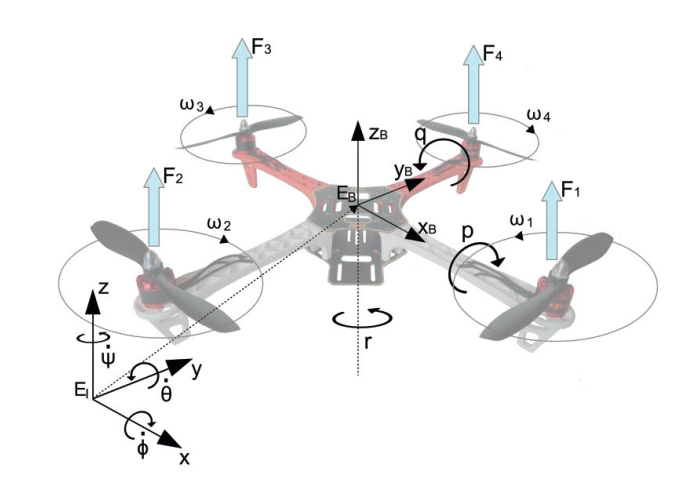
\includegraphics[width=1.0\linewidth]{Images/quad_frame.png}
	\caption{Inertial and body-fixed frame of the quadrotor, showing the Euler and angular velocity angles [?] %TODO CITE
		}
	\label{fig:quad_frame}
\end{figure}


 The rotation from the body frame to the inertial frame can be defined with the matrix

$$\bm{R}=\left[ \begin{array}{ccc}{C_{\psi} C_{\theta}} & {C_{\psi} S_{\theta} S_{\phi}-S_{\psi} C_{\phi}} & {C_{\psi} S_{\theta} C_{\phi}+S_{\psi} S_{\phi}} \\ {S_{\psi} C_{\theta}} & {S_{\psi} S_{\theta} S_{\phi}+C_{\psi} C_{\phi}} & {S_{\psi} S_{\theta} C_{\phi}-C_{\psi} S_{\phi}} \\ {-S_{\theta}} & {C_{\theta} S_{\phi}} & {C_{\theta} C_{\phi}}\end{array}\right]$$

in which $S_{x}=\sin (x)$ and $C_{x}=\cos (x)$. Note that this rotation matrix is orthogonal and thus the rotation matrix from the inertial frame to the body frame is $\bm{R^{-1} = \bm{R^T}}$.

To obtain the angular velocities in the body frame from the angular velocities in the inertial frame, the matrix $\bm{W_\eta}$ should be used:

$\bm{\nu}=\bm{W}_{\eta} \dot{\bm{\eta}}, \hfill \left[ \begin{array}{l}{p} \\ {q} \\ {r}\end{array}\right]=\left[ \begin{array}{ccc}{1} & {0} & {-S_{\theta}} \\ {0} & {C_{\phi}} & {C_{\theta} S_{\phi}} \\ {0} & {-S_{\phi}} & {C_{\theta} C_{\phi}}\end{array}\right] \left[ \begin{array}{c}{\dot{\phi}} \\ {\dot{\theta}} \\ {\dot{\psi}}\end{array}\right]$

Its inverse is the transformation matrix from the body frame to the inertial frame, which will be used later to assemble the quadrotor dynamics:

$\dot{\bm{\eta}}=\bm{W}_{\eta}^{-1} \bm{\nu}$, \hfill $\left[ \begin{array}{c}{\dot{\phi}} \\ {\dot{\theta}} \\ {\dot{\psi}}\end{array}\right]=\left[ \begin{array}{ccc}{1} & {S_{\phi} T_{\theta}} & {C_{\phi} T_{\theta}} \\ {0} & {C_{\phi}} & {-S_{\phi}} \\ {0} & {S_{\phi} / C_{\theta}} & {C_{\phi} / C_{\theta}}\end{array}\right] \left[ \begin{array}{l}{p} \\ {q} \\ {r}\end{array}\right]$

where $T_{x}=\tan (x)$.

As shown in Figure~\ref{fig:quad_frame} and stated in assumption~\ref{as:inertia}, the drone is symmetric with the arms aligned with the body axes. Therefore, the inertia matrix $\textbf{I}$ is diagonal, and $I_{xx} = I_{yy}$:

 $$\boldsymbol{I}=\left[ \begin{array}{ccc}{I_{x x}} & {0} & {0} \\ {0} & {I_{y y}} & {0} \\ {0} & {0} & {I_{z z}}\end{array}\right]$$
 
 \subsection{Quadrotor Dynamics}

The force $f_i$ created by the angular velocity of rotor $i$, denoted with $\omega_i$, in the direction of the rotor axis is:

$$f_{i}=k \omega_{i}^{2}$$

Additionally, torque $\tau_{M_i}$ is created around the rotor axis:

$$\tau_{M_{i}} = b \omega_{i}^{2} + I_{r} \dot{\omega}_{i} $$

where the lift constant is $k$, the drag constant is $b$ and the inertia moment of the rotor is $I_{r}$. As assumption~\ref{as:Ir} considered, the rotor's inertia is small, and $\dot{\omega}_{i}$ is also usually small. Therefore, this term can be omitted.

The rotors create thrust $T$ in the direction of the body z-axis, and torque $\bm{\tau_B}$ consists of torques $\tau_\phi, \tau_\theta, \tau_\psi$ in the direction of the corresponding body frame angles:

$$T=\sum_{i=1}^{4} f_{i}=k \sum_{i=1}^{4} \omega_{i}^{2}, \quad \quad \boldsymbol{T}^{B}=\left[ \begin{array}{c}{0} \\ {0} \\ {T}\end{array}\right]$$

$$
\boldsymbol{\tau}_{B}=\left[ \begin{array}{c}{\tau_{\phi}} \\ {\tau_{\theta}} \\ {\tau_{\psi}}\end{array}\right]=
\left[ \begin{array}{c}{l k\left(-\omega_{2}^{2}+\omega_{4}^{2}\right)} \\ {l k\left(-\omega_{1}^{2}+\omega_{3}^{2}\right)} \\ {\sum_{i=1}^{4} \tau_{M_{i}}}\end{array}\right]
$$

in which l is the distance between the rotor and the center of mass of the quadcopter.

The Newton-Euler equations for the quadrotor are:

$$m \ddot{\boldsymbol{\xi}}=\boldsymbol{G}+\boldsymbol{R} \boldsymbol{T}_{B}$$

$$\left[ \begin{array}{c}{\ddot{x}} \\ {\ddot{y}} \\ {\ddot{z}}\end{array}\right]=-g \left[ \begin{array}{l}{0} \\ {0} \\ {1}\end{array}\right]+\frac{T}{m} \left[ \begin{array}{c}{C_{\psi} S_{\theta} C_{\phi}+S_{\psi} S_{\phi}} \\ {S_{\psi} S_{\theta} C_{\phi}-C_{\psi} S_{\phi}} \\ {C_{\theta} C_{\phi}}\end{array}\right]$$

where g is Earth's gravity, 9.81 $m/s^2$.
 
% As stated in assumption~\ref{as:Ir}, 

%Problem, dynamics and assumptions. Minimize integral of dt from t0 to tf = tf subject to the dynamics, gates, starting point and constraints (zmin).



\section{RESULTS}\label{s:exp}

Explain solved using GPOPS.

  

\section{CONCLUSIONS}\label{s:conclusions}

Conclusions

\addtolength{\textheight}{-12cm}   % This command serves to balance the column lengths
                                  % on the last page of the document manually. It shortens
                                  % the textheight of the last page by a suitable amount.
                                  % This command does not take effect until the next page
                                  % so it should come on the page before the last. Make
                                  % sure that you do not shorten the textheight too much.

%%%%%%%%%%%%%%%%%%%%%%%%%%%%%%%%%%%%%%%%%%%%%%%%%%%%%%%%%%%%%%%%%%%%%%%%%%%%%%%%
%%%%%%%%%%%%%%%%%%%%%%%%%%%%%%%%%%%%%%%%%%%%%%%%%%%%%%%%%%%%%%%%%%%%%%%%%%%%%%%%
\section*{APPENDIX}

Nothing...

Citation: \cite{IEEEexample:article_typical}.

%%%%%%%%%%%%%%%%%%% CHECK BIB MANUAL %%%%%%%%%%%%%%%%%%%%%%%%%%%%%%%%%%%%%%%%%%%%%%%%%%%%%%%%%%%%%%%%%
%\begin{thebibliography}{99}

\balance

\makeatletter
\def\endthebibliography{%
	\def\@noitemerr{\@latex@warning{Empty `thebibliography' environment}}%
	\endlist
}
\makeatother

\bibliographystyle{unsrt}
\bibliography{IEEEexample}
%\end{thebibliography}
%%%%%%%%%%%%%%%%%%%%%%%%%%%%%%%%%%%%%%%%%%%%%%%%%%%%%%%%%%%%%%%%%%%%%%%%%%%%%%%%%%%%%%%%%%%%%%%%%%%%%%

\end{document}
